% !TeX root = ../../main.tex
\section{Mechanical drawings}
\label{app:reactor-drawings}
\subsection{3D mechanical design and engineering drawings}
\label{app:engineeringdesign}
All dimensions are in the units of mm.

\begin{figure}
    \centering
    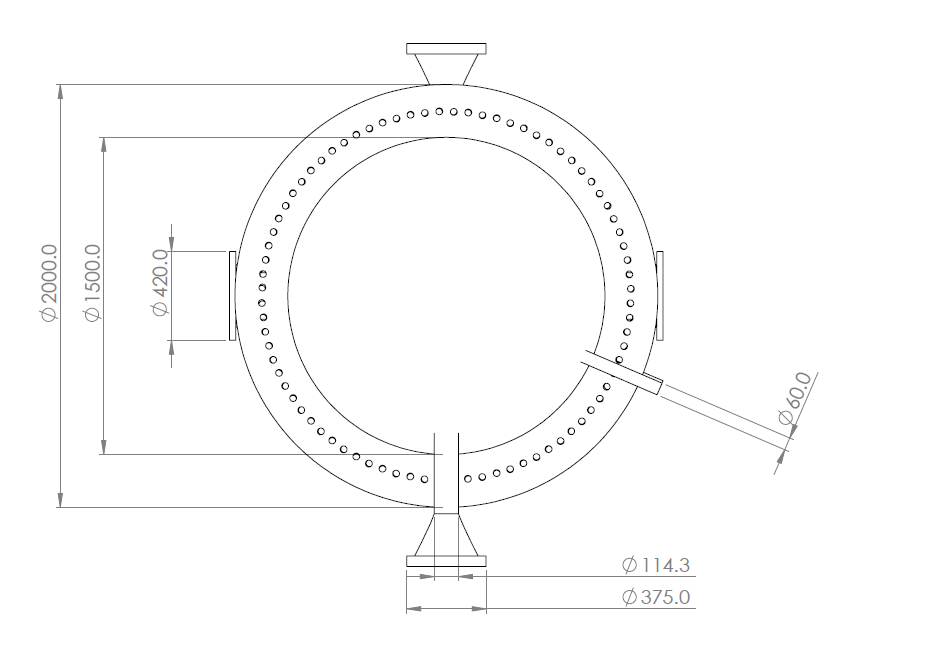
\includegraphics[width=0.6\linewidth]{chapters/2-reaction/figures/FYD reactor bottom view with calc.PNG}
    \caption{Bottom view of the reactor}
    \label{fig:reactorbottom}
    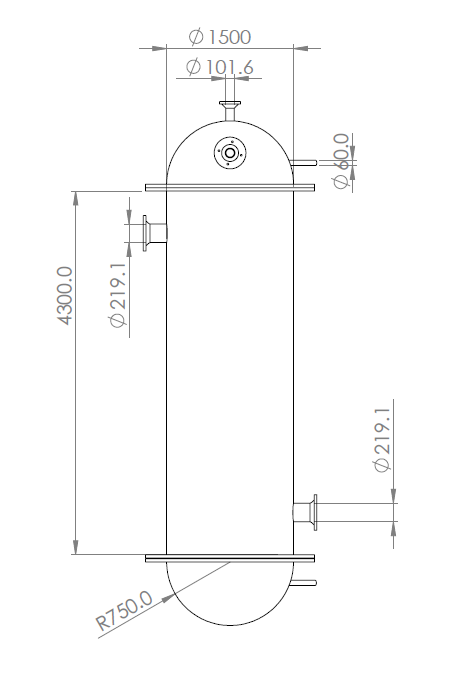
\includegraphics[width=0.49\linewidth]{chapters/2-reaction/figures/FYD reactor right view with calc.PNG}
    \caption{Right view of the reactor}
    \label{fig:reactorright}
    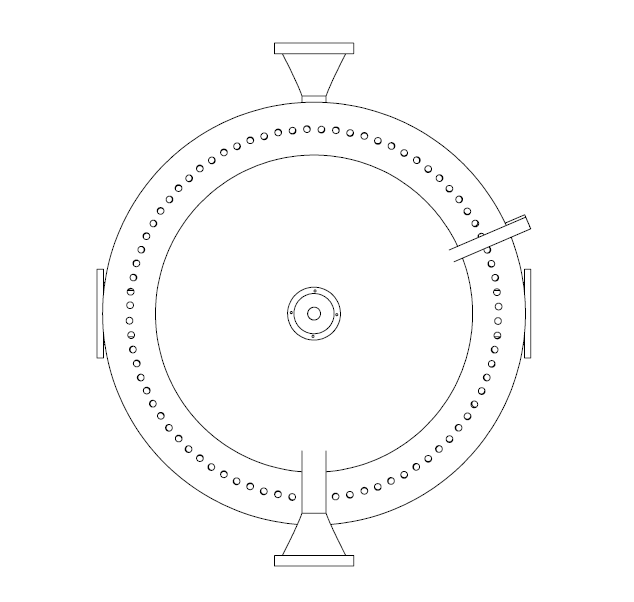
\includegraphics[width=0.49\linewidth]{chapters/2-reaction/figures/FYD reactor top view.PNG}
    \caption{Top view of the reactor}
    \label{fig:reactortop}
\end{figure}

\begin{figure}[p]
    
    \begin{minipage}{\linewidth}
        \centering
        \begin{subfigure}{0.42\linewidth}
            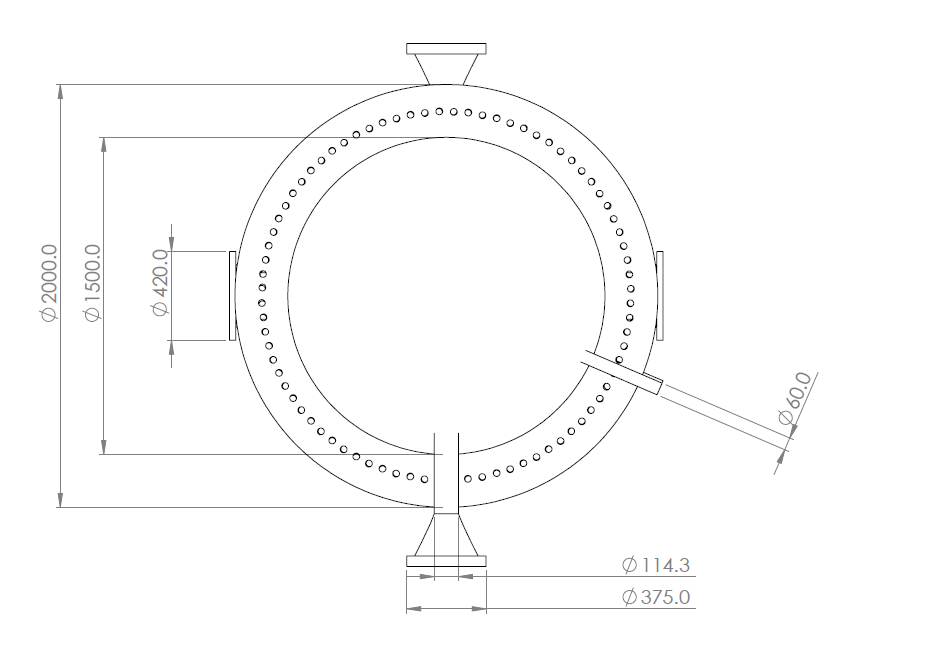
\includegraphics[width=\linewidth, scale=0.5]{chapters/2-reaction/figures/FYD reactor bottom view with calc.PNG}
            \caption{Rate of Toluene reaction}
            \label{fig:comsol-performance:r_TOL}
        \end{subfigure}\hspace{\floatsep}
        \begin{subfigure}{0.42\linewidth}
            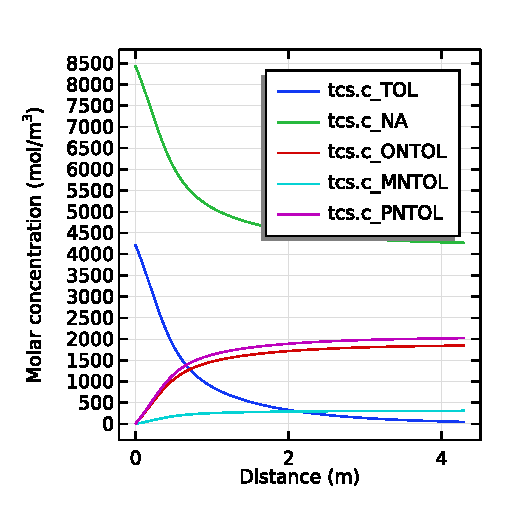
\includegraphics[width=\linewidth, scale=0.5]{figures/concentration.eps}
            \caption{Concentration profile within reactor}
            \label{fig:comsol-performance:concentration}
        \end{subfigure}
        \caption{Reactor performance}
        \label{fig:comsol-performance}
    \end{minipage}
    \vspace{\floatsep}
    
\end{figure}